\documentclass{article}
\usepackage{amsmath}
\usepackage{amssymb}
\usepackage{graphicx}
\newcommand{\bld}[1]{\boldsymbol{#1}}

\begin{document}

\title{MATH520 Homework 1}
\author{Fernando}
\date{\today}
\maketitle

\section*{Exercise 1.5}
Suppose that you are shown four cards, laid out in a row. Each card has a letter on one side and a number on the other. On the visible side of the cards are printed the symbols

\begin{center}
S \quad 8 \quad 3 \quad A
\end{center}

Determine which cards should you turn over to decide if the following rule is true or false: "If there is a vowel on one side of the card, then there is an even number on the other side."

\textbf{Solution:}

If a card has a vowel we should turn it over to check that the other side has
an even number. Consonants are not mentioned in the rule so what is on the
other side of a consonant is irrelevant. Odd numbers should be turned over to
make sure there is not a vowel on the other side and even numbers are OK no
matter what is on the other side so no need to turn them over.

\textbf{Answer:} 3 and A.
\section*{Exercise 2.10}
Show that for any two vectors $\boldsymbol{x},\boldsymbol{y}\in\mathbb{R}^n$,
$|||\boldsymbol{x}||-||\boldsymbol{y}||| \leq
||\boldsymbol{x}-\boldsymbol{y}||$.

\textbf{Solution:}

\[
||\bld{x}||=||\bld{x}-\bld{y}+\bld{y}|| \leq ||\bld{x}-\bld{y}|| + ||\bld{y}||
\]
then,
\begin{equation}
||\bld{x}||-||\bld{y}|| \leq ||\bld{x}-\bld{y}||.
\end{equation}
Notice that since $\bld{x}$ and  $\bld{y}$ are arbitrary vectors by switching
them we also get:
\begin{equation}
||\bld{y}||-||\bld{x}|| \leq ||\bld{y}-\bld{x}||=||\bld{x}-\bld{y}||.
\end{equation}
Multiplying (2) by -1 we get:
\begin{equation}
||\bld{x}||-||\bld{y}|| \geq -||\bld{x}-\bld{y}||.
\end{equation}
Together (1) and (3) are equivalent to:
\[
	|||\bld{x}||-||\bld{y}|||\leq ||\bld{x}-\bld{y}||.
\]
\section*{Exercise 3.6}
Let $\lambda_1,\dots,\lambda_n$ be the eigenvalues of the matrix $A\in
\mathbb{R}^{n\times n}$. Show that the eigenvalues of the matrix $I_n -A$ are
$1-\lambda_1,\dots,1-\lambda_n$.

\textbf{Solution:}

Let $v_i$ be an eigenvector associated with the eigenvalue $\lambda_i$, then
\[
	(I_n-A)v_i=v_i-Av_i=v_i-\lambda_iv_i=(1-\lambda_i)v_i.
\]
So the eigenvalues of $I_n-A$ are indeed $(1-\lambda_i)$.
\section*{Exercise 3.17}
Consider the matrix
\[ Q=
\begin{bmatrix}
0 & 1 & 1\\	
1 & 0 & 1\\
1 & 1 & 0
\end{bmatrix}.
\]
a. Is the matrix positive definite, negative definite, or indefinite?

\textbf{Solution 1:}

Explicitly computing the eigenvalues using Sarrus' rule to find the characteristic
polynomial $(-\lambda^3+3\lambda+2)$ and then finding its roots gives us:\\
$\lambda_1=-1,\lambda_2=-1,\lambda_3=2$. So it is indefinite.

\textbf{Solution 2:}

The leading principal minors are: $\Delta_1=0$, $\Delta_2=-1$,
$\Delta_3=\det(Q)=2$.

so by Sylvester's criterion this matrix is indefinite.
\section*{Exercise 5.7}
Let $x(t)=[e^t+t^3,t^2,t+1]^T$, $t\in \mathbb{R}$, and $f(x)=x_1^3x_2x_3^2 +
x_1x_2 + x_3$,\\
$x=[x_1,x_2,x_3]^T\in \mathbb{R}^3$.\\
Find $\frac{d}{dt}f(x(t))$ in terms of $t$.

\textbf{Solution:}

According to the chain rule the derivative is
\[
\frac{d}{dt}f(x(t))=\nabla f(x(t))\cdot x'(t),
\]
where $x'(t)$ is a vector obtained by differentiating $x(t)$ entry-wise.

$\nabla f$ is:
\[
\begin{bmatrix}
	3x_1^2x_2x_3^2+x_2\\
	x_1^3x_3^2 + x_1\\
	2x_1^3x_2x_3+1\\
\end{bmatrix}.
\]
Then $\nabla f(x(t))$ is:
\[
\begin{bmatrix}
	3(e^t+t^3)^2(t^2)(t+1)^2+(t^2)\\
	(e^t+t^3)^3(t+1)^2 + (e^t+t^3)\\
	2(e^t+t^3)^3(t^2)(t+1)+1\\
\end{bmatrix}.
\]

So the result is:
\begin{multline*}
\begin{bmatrix}
	3(e^t+t^3)^2(t^2)(t+1)^2+(t^2)\\
	(e^t+t^3)^3(t+1)^2 + (e^t+t^3)\\
	2(e^t+t^3)^3(t^2)(t+1)+1\\
\end{bmatrix}
\cdot
\begin{bmatrix}
	e^t+3t^2\\
	2t\\
	1\\
\end{bmatrix}
=\\
(e^t+3t^2)(3(e^t+t^3)^2t^2(t+1)^2 + t^2)\\
+2t((e^t+t^3)^3(t+1)^2 + (e^t+t^3))\\
+2(e^t+t^3)^3(t^2)(t+1)+1.
\end{multline*}
\section*{Exercise 5.10}
Let
\begin{align*}
	f_1(x_1,x_2)&=x_1^2-x_2^2,\\
	f_2(x_1,x_2)&=2x_1x_2.
\end{align*}

Sketch the level sets associated with $f_1(x_1,x_2)=12$ and $f_2(x_1,x_2)=16$
on the same diagram. Indicate on the diagram the values of
$\boldsymbol{x}=[x_1,x_2]^T$ for which
$\boldsymbol{f}(\boldsymbol{x})=[f_1(x_1,x_2),f_2(x_1,x_2)]^T=[12,16]^T$.

\textbf{Solution:}

We have to plot $x_1^2-x_2^2=12$ and $2x_1x_2=16$, then for the condition
$\boldsymbol{f}(\boldsymbol{x})=[12,16]^T$ to be true we need to find the
points at the intersection of the 2 curves.

\begin{figure}[ht]
	\caption{Level sets of $f_1$(dotted, red) and $f_2$(continuous, blue)}
	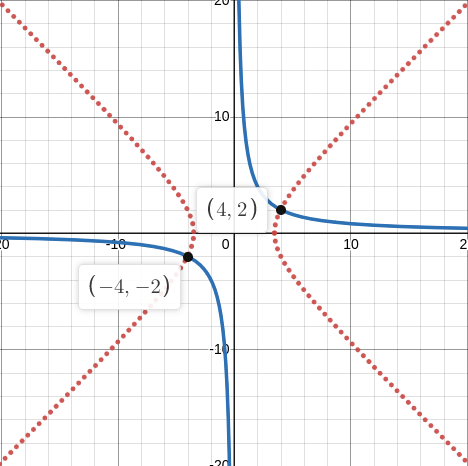
\includegraphics[width=\textwidth]{sketch-hw-1.png}
\end{figure}
\end{document}
